Input to the Streamflow Routing (SFR) Package is read from the file that has type ``SFR6'' in the Name File. Any number of SFR Packages can be specified for a single groundwater flow model; however, water cannot be routed between reaches in separate packages except in cases where the MVR Package is used to route water between separate packages. Reaches can be specified to have a wide-rectangular cross-section or an irregular cross-section with an arbitrary number of station-height points (added in version 6.3.0). Irregular cross-sections are discussed in the \hyperref[sec:n-point]{Streamflow Routing Package Cross-Section Table Input File} section.

Reach connectivity must be explicitly specified for this version of the SFR Package, unlike the abbreviated SFR Package segment connectivity specified in previous versions of MODFLOW. Explicit specification of reach connectivity has been adopted to facilitate better validation of stream network connectivity by the program. Explicit reach connectivity means that a reach must be specified as an upstream connection for all downstream connections to the reach. Downstream connections for a reach are denoted with a negative reach number. Flow in a reach is unidirectional, always flowing from the upstream end to the downstream end of a reach. An example of the reach connectivity for a hypothetical stream network is shown in figure~\ref{fig:sfr-connectivity}.

\begin{figure}[ht]
	\centering
	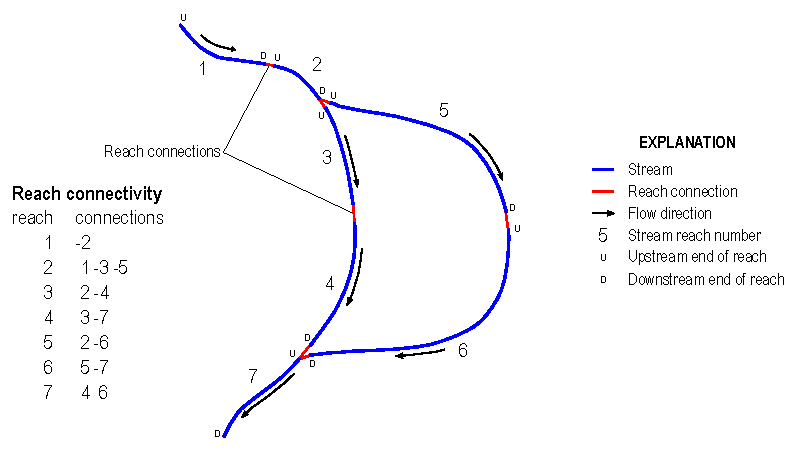
\includegraphics[scale=1.0]{../Figures/sfr-connectivity}
	\caption[Illustration of a simple stream network having seven reaches with a junction having two reaches, a confluence of two reaches, and the resulting reach connectivity]{Simple stream network having seven reaches with a junction having two reaches, a confluence of two reaches, and the resulting reach connectivity. Downstream connections for a reach must include the reach as an upstream connection for all downstream connections to the reach. Downstream connections for a  reach are denoted with a negative reach number}
	\label{fig:sfr-connectivity}
\end{figure}

\vspace{5mm}
\subsubsection{Structure of Blocks}

\vspace{5mm}
\noindent \textit{FOR EACH SIMULATION}
\lstinputlisting[style=blockdefinition]{./mf6ivar/tex/gwf-sfr-options.dat}
\lstinputlisting[style=blockdefinition]{./mf6ivar/tex/gwf-sfr-dimensions.dat}
\lstinputlisting[style=blockdefinition]{./mf6ivar/tex/gwf-sfr-packagedata.dat}

\vspace{5mm}
\noindent \textit{CROSSSECTIONS BLOCK IS OPTIONAL}
\lstinputlisting[style=blockdefinition]{./mf6ivar/tex/gwf-sfr-crosssections.dat}

\lstinputlisting[style=blockdefinition]{./mf6ivar/tex/gwf-sfr-connectiondata.dat}

\vspace{5mm}
\noindent \textit{IF ndv IS GREATER THAN ZERO FOR ANY REACH}
\lstinputlisting[style=blockdefinition]{./mf6ivar/tex/gwf-sfr-diversions.dat}

\vspace{5mm}
\noindent \textit{INITIALSTAGES BLOCK IS OPTIONAL}
\lstinputlisting[style=blockdefinition]{./mf6ivar/tex/gwf-sfr-initialstages.dat}

\vspace{5mm}
\noindent \textit{FOR ANY STRESS PERIOD}
\lstinputlisting[style=blockdefinition]{./mf6ivar/tex/gwf-sfr-period.dat}
\advancedpackageperioddescription{reach}{reaches}

\vspace{5mm}
\subsubsection{Explanation of Variables}
\begin{description}
\input{./mf6ivar/tex/gwf-sfr-desc.tex}
\end{description}

\vspace{5mm}
\subsubsection{Example Input File}
\lstinputlisting[style=inputfile]{./mf6ivar/examples/gwf-sfr-example.dat}

\vspace{5mm}
\subsubsection{Available observation types}
Streamflow Routing Package observations include reach stage and all of the terms that contribute to the continuity equation for each stream reach. Additional SFR Package observations include the sum of inflows from upstream reaches and from mover terms (\texttt{upstream-flow}) and downstream outflow from a reach prior to diversions and the mover package (\texttt{downstream-flow}). The data required for each SFR Package observation type is defined in table~\ref{table:gwf-sfrobstype}. Negative and positive values for \texttt{sfr} observations represent a loss from and gain to the GWF model, respectively. For all other flow terms, negative and positive values represent a loss from and gain from the SFR package, respectively.

\FloatBarrier
\begin{longtable}{p{2cm} p{2.75cm} p{2cm} p{1.25cm} p{7cm}}
\caption{Available SFR Package observation types} \tabularnewline

\hline
\hline
\textbf{Stress Package} & \textbf{Observation type} & \textbf{ID} & \textbf{ID2} & \textbf{Description} \\
\hline
\endfirsthead

\captionsetup{textformat=simple}
\caption*{\textbf{Table \arabic{table}.}{\quad}Available SFR Package observation types.---Continued} \\

\hline
\hline
\textbf{Stress Package} & \textbf{Observation type} & \textbf{ID} & \textbf{ID2} & \textbf{Description} \\
\hline
\endhead


\hline
\endfoot

SFR & stage & ifno or boundname & -- & Surface-water stage in a stream-reach boundary. If boundname is specified, boundname must be unique for each reach. \\
SFR & ext-inflow & ifno or boundname & -- & Inflow into a stream-reach from an external boundary for a stream-reach or a group of stream-reaches. \\
SFR & inflow & ifno or boundname & -- & Inflow into a stream-reach from upstream reaches for a stream-reach or a group of stream-reaches. \\
SFR & from-mvr & ifno or boundname & -- & Inflow into a stream-reach from the MVR package for a stream-reach or a group of stream-reaches. \\
SFR & rainfall & ifno or boundname & -- & Rainfall rate applied to a stream-reach or a group of stream-reaches. \\
SFR & runoff & ifno or boundname & -- & Runoff rate applied to a stream-reach or a group of stream-reaches. \\
SFR & sfr & ifno or boundname & -- & Simulated flow rate for a stream-reach and its aquifer connection for a stream-reach or a group of stream-reaches. \\
SFR & evaporation & ifno or boundname & -- & Simulated evaporation rate from a stream-reach or a group of stream-reaches. \\
SFR & outflow & ifno or boundname & -- & Outflow from a stream-reach to downstream reaches for a stream-reach or a group of stream-reaches. \\
SFR & ext-outflow & ifno or boundname & -- & Outflow from a stream-reach to an external boundary for a stream-reach or a group of stream-reaches. \\
SFR & to-mvr & ifno or boundname & -- & Outflow from a stream-reach that is available for the MVR package for a stream-reach or a group of stream-reaches. \\
SFR & upstream-flow & ifno or boundname & -- & Upstream flow for a stream-reach or a group of stream-reaches from upstream reaches and the MVR package. \\
SFR & downstream-flow & ifno or boundname & -- & Downstream flow for a stream-reach or a group of stream-reaches prior to diversions and the MVR package. \\
SFR & depth & ifno or boundname & -- & Surface-water depth in a stream-reach boundary. If boundname is specified, boundname must be unique for each reach. \\
SFR & wet-perimeter & ifno or boundname & -- & Wetted perimeter in a stream-reach boundary. If boundname is specified, boundname must be unique for each reach. \\
SFR & wet-area & ifno or boundname & -- & Wetted cross-section area in a stream-reach boundary. If boundname is specified, boundname must be unique for each reach. \\
SFR & wet-width & ifno or boundname & -- & Wetted top width in a stream-reach boundary. If boundname is specified, boundname must be unique for each reach. \\


\label{table:gwf-sfrobstype}
\end{longtable}
\FloatBarrier

\vspace{5mm}
\subsubsection{Example Observation Input File}
\lstinputlisting[style=inputfile]{./mf6ivar/examples/gwf-sfr-example-obs.dat}

\newpage
\subsection{Streamflow Routing Package Cross-Section Table Input File} \label{sec:n-point}

The approach used to represent irregular cross-sections in the SFR Package is a generalization of the 8-point cross-section available in the SFR Package for previous versions of MODFLOW \citep{modflowsfr1pack}. The station-height data for irregular cross-sections is specified as xfraction and height data (fig.~\ref{fig:sfr-n-point}), which is converted to station position using the specified reach width (RWID) and elevation using the specified bottom elevation of the reach (RTP). Fraction values were specified for the station data to maintain use of the specified reach width for reaches using irregular cross-sections. Furthermore, use of a maximum xfraction value less than or greater than one allows users to vary the width of a reach during a simulation.

Manning's roughness coefficient fractions can optionally be specified with the xfraction-height data for a irregular cross-section to represent roughness coefficient variations in a channel (for example, different channel and overbank Manning's roughness coefficients). When Manning's coefficient fractions are specified, the streamflow is calculated for each segment of the cross-section and summed to calculate the total streamflow for a reach; this is the same approach used in the SFR Package for previous versions of MODFLOW \citep{modflowsfr1pack} to calculate the stream flow for the left bank, defined channel, and right bank. Fraction values are specified for irregular cross-section Manning's roughness coefficient data in order to allow users to also set Manning's roughness coefficients in the stress period data and using timeseries.


\begin{figure}[ht]
	\centering
	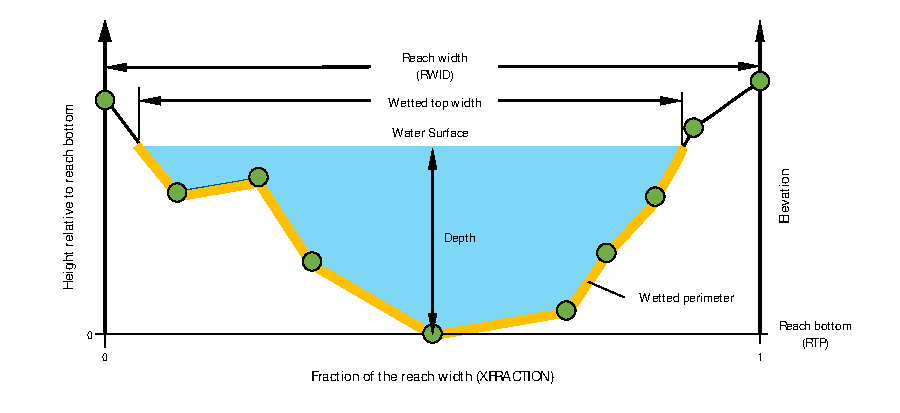
\includegraphics[scale=1.0]{../Figures/n-point-cross-section}
	\caption[Illustration of a irregular cross section used to compute depth, wetted top width, wetted perimeter, and wetted cross-sectional area for a stream reach]{Irregular cross section used to compute depth, wetted top width, wetted perimeter, and wetted cross-sectional area for a stream reach for the case where the maximum XFRACTION is one}
	\label{fig:sfr-n-point}
\end{figure}

Where irregular cross sections are used to define cross-sectional stream geometries, the wetted perimeter used in Manning’s equation [Equation 7-7, \cite{modflow6gwf}] depends on the number of points defining the cross section and the simulated stage.  Using only the minimum number of points (i.e., 2-point cross section), \mf does not include perimeter lengths above the uppermost defined points in the wetted perimeter calculations. For example, the 2-point cross sections shown in fig.~\ref{fig:sfr-n-point-wp}A-C depict the cross-sectional areas (light blue) and wetted perimeters (orange) calculated by the SFR package and used in \cite{modflow6gwf} (Equation 7-7).  In applications where the intent is for the wetted perimeter to include the entire lengths of wetted sides, additional points above the maximum anticipated stage should be defined (fig.~\ref{fig:sfr-n-point-wp}D).  Note that when the simulated stream stage rises above the points representing the top of the channel, the additional cross-sectional flow area above the defined points will be accounted for but the corresponding wetted perimeter will not extend above the defined points (fig.~\ref{fig:sfr-n-point-wp}E,F).


\begin{figure}[ht]
	\centering
	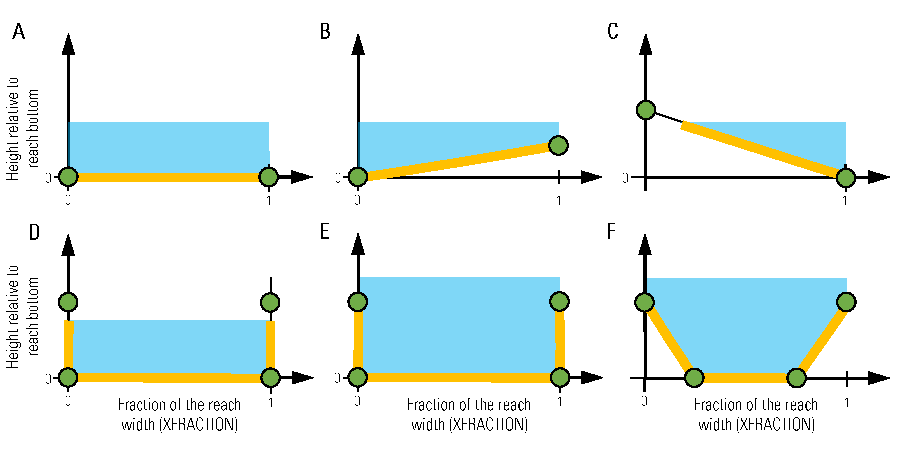
\includegraphics[scale=1.0]{../Figures/n-point-cross-section-wetted-perimeter}
	\caption[Illustrations of variously defined n-point cross-sections that show how wetted perimeter will vary depending on the stage and the number of points used to define the cross-section]{Example irregular cross-section geometries showing the corresponding wetted perimeter based on the number of points that define a cross-section and the simulated stage.  (A-C) Wetted perimeters (orange lines) for variously configured 2-point cross-sections.  (D-F) Wetted perimeters for variously configured 4-point cross-sections}
	\label{fig:sfr-n-point-wp}
\end{figure}

Cross-Section tables are specified by including file names in the CROSSSECTIONS or PERIOD blocks of the SFR Package for specific reaches.  These file names correspond to a Streamflow Routing cross-section table input file.  The format of the Streamflow Routing cross-section table input file is described here.

\vspace{5mm}
\subsubsection{Structure of Blocks}
\vspace{5mm}

\lstinputlisting[style=blockdefinition]{./mf6ivar/tex/utl-sfrtab-dimensions.dat}
\lstinputlisting[style=blockdefinition]{./mf6ivar/tex/utl-sfrtab-table.dat}
\vspace{5mm}

\vspace{5mm}
\subsubsection{Explanation of Variables}
\begin{description}
\input{./mf6ivar/tex/utl-sfrtab-desc.tex}
\end{description}

\subsubsection{Example Input File}
\lstinputlisting[style=inputfile]{./mf6ivar/examples/utl-sfrtab-example.dat}

